\section{SVD 是什么}

奇异值分解（Singular Value Decomposition, SVD）是线性代数里最像“显微镜”的分解：
它不要求矩阵是方阵，不要求矩阵可逆，也不要求矩阵可对角化，却仍然能把任意线性映射
\[
    A:\mathbb{R}^n\to\mathbb{R}^m
\]
拆成三个结构极其干净的部分：
\[
    A = U\Sigma V^T.
\]
其中 $U\in\mathbb{R}^{m\times m}$ 与 $V\in\mathbb{R}^{n\times n}$ 是正交矩阵
（orthogonal matrix），满足 $U^TU=I_m$、$V^TV=I_n$；$\Sigma\in\mathbb{R}^{m\times n}$
是非负“对角”矩阵，即
\[
    \Sigma =
    \begin{bmatrix}
        \sigma_1 &          &        &          \\
                 & \sigma_2 &        &          \\
                 &          & \ddots &          \\
                 &          &        & \sigma_p \\
                 &          &        &
    \end{bmatrix},
    \qquad
    p=\min\{m,n\},
    \qquad
    \sigma_1\ge \sigma_2\ge \cdots\ge \sigma_p\ge 0.
\]
这些非负数 $\sigma_i$ 称为 $A$ 的奇异值（singular value）。$U$ 的列向量称为左奇异向量
（left singular vector），$V$ 的列向量称为右奇异向量（right singular vector）。

如果矩阵的秩（rank）为 $r$，则恰有 $r$ 个正奇异值。此时也常写成紧 SVD
（thin SVD / economy SVD）：
\[
    A = U_r\Sigma_r V_r^T
    = \sum_{i=1}^{r}\sigma_i u_i v_i^T,
\]
其中 $U_r=[u_1,\ldots,u_r]\in\mathbb{R}^{m\times r}$，
$V_r=[v_1,\ldots,v_r]\in\mathbb{R}^{n\times r}$，
$\Sigma_r=\operatorname{diag}(\sigma_1,\ldots,\sigma_r)$。
这个求和形式非常关键：它说明矩阵可以被看作 $r$ 个秩一矩阵（rank-one matrix）的叠加。
每一项 $\sigma_i u_i v_i^T$ 都是一种方向性的能量模式；$\sigma_i$ 越大，该模式越重要。

\subsection{几何图像：旋转、缩放、再旋转}

从几何上看，SVD 把任何线性映射拆成三步：
\[
    x
    \xrightarrow{\;V^T\;}
    V^Tx
    \xrightarrow{\;\Sigma\;}
    \Sigma V^Tx
    \xrightarrow{\;U\;}
    U\Sigma V^Tx.
\]
第一步 $V^T$ 只是改变输入空间中的正交坐标系；第二步 $\Sigma$ 沿坐标轴缩放，
并可能把某些方向压扁到 $0$；第三步 $U$ 再改变输出空间中的正交坐标系。
因此，SVD 的核心断言可以说成：

\begin{quote}
    任意矩阵都可以被理解为：输入空间的一次正交重标定、坐标轴方向的非负缩放、
    输出空间的一次正交重标定。
\end{quote}

这比“矩阵可以分解成三个矩阵”更有信息量。因为正交变换保持长度与角度，不引入数值放大；
真正改变几何尺度的全部信息，都被集中到非负奇异值 $\sigma_i$ 里。于是立即得到
\[
    \|A\|_2 = \sigma_1,\qquad
    \|A\|_F^2 = \sum_{i=1}^{p}\sigma_i^2,\qquad
    \kappa_2(A)=\frac{\sigma_1}{\sigma_r}
    \quad (A\text{ 满列秩或可逆时}),
\]
其中 $\|\cdot\|_2$ 是谱范数（spectral norm），$\|\cdot\|_F$ 是 Frobenius 范数
（Frobenius norm），$\kappa_2$ 是二范数条件数（condition number）。
这也是 SVD 在数值计算中拥有特殊地位的原因：它把“一个线性系统有多病态”这件事转化为
奇异值谱（singular spectrum）的形状。

\begin{figure}[htbp]
    \centering
    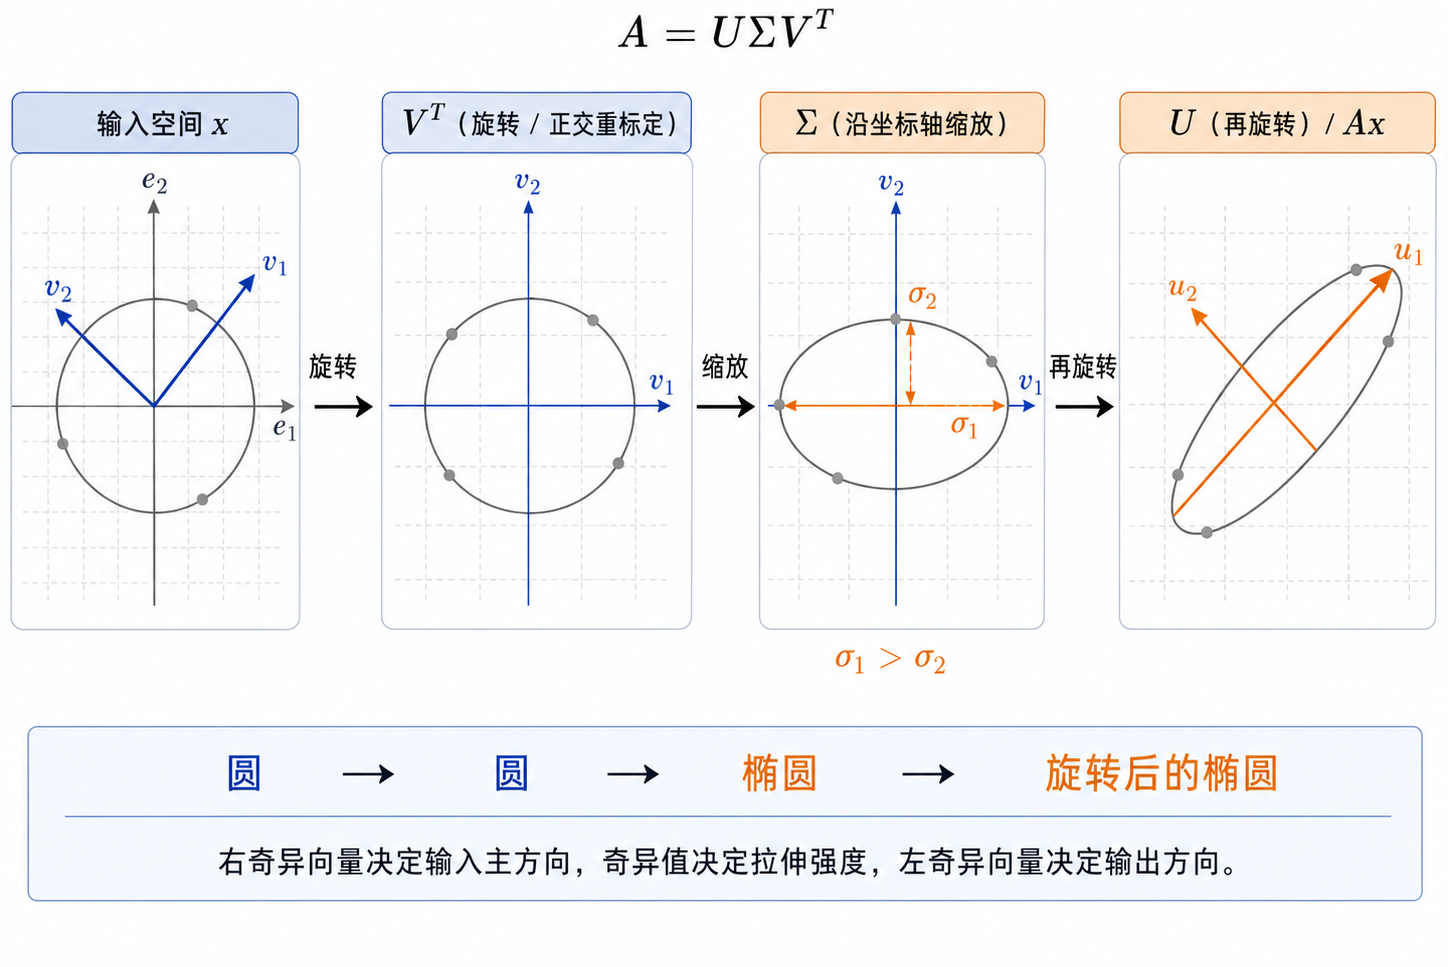
\includegraphics[width=0.92\textwidth]{figures/what-is-svd.png}
\end{figure}

\subsection{为什么 SVD 到处都在}

SVD 的应用并不是偶然拼贴出来的；它们都来自同一个结构事实：
SVD 同时给出矩阵的正交基、尺度谱与最优低秩逼近。下面这些场景看似分散，其实共享同一套数学骨架。

\paragraph{最小二乘与伪逆。}
在线性最小二乘（linear least squares）问题
\[
    \min_x \|Ax-b\|_2
\]
中，若 $A=U\Sigma V^T$，则 Moore--Penrose 伪逆（pseudoinverse）为
\[
    A^+ = V\Sigma^+U^T,
    \qquad
    \Sigma^+_{ii} =
    \begin{cases}
        1/\sigma_i, & \sigma_i>0, \\
        0,          & \sigma_i=0.
    \end{cases}
\]
于是最小范数解（minimum-norm solution）可以写成 $x_\star=A^+b$。这一表达式把病态性完全暴露出来：
当某些 $\sigma_i$ 很小时，$1/\sigma_i$ 会放大噪声。因此截断 SVD（truncated SVD）和 Tikhonov
正则化（Tikhonov regularization）都可以被理解为对小奇异值方向的抑制。

\paragraph{低秩近似与压缩。}
Eckart--Young--Mirsky 定理（Eckart--Young--Mirsky theorem）说明，若
\[
    A_k=\sum_{i=1}^{k}\sigma_i u_i v_i^T,
\]
则 $A_k$ 是所有秩不超过 $k$ 的矩阵里对 $A$ 的最优逼近：
\[
    A_k
    \in
    \arg\min_{\operatorname{rank}(B)\le k}\|A-B\|_2,
    \qquad
    \|A-A_k\|_2=\sigma_{k+1},
\]
并且在 Frobenius 范数下也最优：
\[
    \|A-A_k\|_F
    =
    \left(\sum_{i=k+1}^{p}\sigma_i^2\right)^{1/2}.
\]
图像压缩、推荐系统、潜在语义分析（latent semantic analysis）和矩阵补全（matrix completion）
都在不同外衣下使用这一事实：保留大奇异值，丢弃小奇异值，就能保留主结构而过滤细节或噪声。

\paragraph{主成分分析。}
主成分分析（Principal Component Analysis, PCA）本质上是中心化数据矩阵的 SVD。
若 $X\in\mathbb{R}^{N\times d}$ 的每一行是一个样本，且各列已经去均值，则
\[
    X=U\Sigma V^T
\]
中的 $V$ 给出特征空间中的主方向，$\sigma_i^2/(N-1)$ 是样本协方差矩阵
$X^TX/(N-1)$ 的特征值。换句话说，PCA 不是另一门魔法；它是 SVD 对数据云几何形状的读谱。

\paragraph{信号、控制与科学计算。}
在信号处理中，小奇异值往往对应低能量或噪声方向；在控制理论中，奇异值描述系统在不同方向上的增益；
在偏微分方程（partial differential equation）离散化与反问题（inverse problem）中，
奇异值衰减速度揭示问题的适定性（well-posedness）。在高性能计算里，SVD 又是许多鲁棒算法的
基础构件：秩判定、子空间迭代、正交化、压缩存储和误差估计都绕不开它。

\paragraph{机器学习与大模型。}
现代机器学习中，SVD 出现在权重矩阵压缩、低秩适配（Low-Rank Adaptation, LoRA）、
谱归一化（spectral normalization）、表示分析、嵌入空间诊断等任务中。尤其当矩阵规模巨大时，
完整 SVD 往往太贵，研究者会转向随机 SVD（randomized SVD）、块 Krylov 方法（block Krylov method）
或 GPU 上的 Jacobi / QR / divide-and-conquer 变体。我们这个项目实现单边雅可比 SVD
（one-sided Jacobi SVD），正是站在“高精度正交化”和“并行列变换”之间寻找工程平衡。

\subsection{定理：任意实矩阵都存在 SVD}

\paragraph{定理陈述。}
对任意 $A\in\mathbb{R}^{m\times n}$，存在正交矩阵
$U\in\mathbb{R}^{m\times m}$、$V\in\mathbb{R}^{n\times n}$，以及非负对角矩阵
$\Sigma\in\mathbb{R}^{m\times n}$，使得
\[
    A=U\Sigma V^T.
\]
若允许复矩阵 $A\in\mathbb{C}^{m\times n}$，同样结论成立，只需把转置 $T$ 替换为共轭转置
（conjugate transpose）$*$，把正交矩阵替换为酉矩阵（unitary matrix）。

\paragraph{证明思路。}
真正需要证明的是：能否在输入空间中找到一组正交方向
$v_i$，使得 $Av_i$ 在输出空间中也两两正交。若能做到，那么 $Av_i$ 的长度就是奇异值，
归一化后的 $Av_i$ 就是左奇异向量。这个想法把问题从一般矩阵 $A$ 拉回到对称半正定矩阵
$A^TA$，而后者可以被谱定理（spectral theorem）处理。

\paragraph{证明。}
令
\[
    B=A^TA\in\mathbb{R}^{n\times n}.
\]
则 $B$ 是实对称矩阵，并且对任意 $x\in\mathbb{R}^n$，
\[
    x^TBx=x^TA^TAx=\|Ax\|_2^2\ge 0,
\]
所以 $B$ 是半正定矩阵（positive semidefinite matrix）。由实对称矩阵谱定理，存在正交矩阵
$V=[v_1,\ldots,v_n]$ 和实数 $\lambda_1,\ldots,\lambda_n$，使得
\[
    Bv_i=\lambda_i v_i,\qquad
    V^TBV=\operatorname{diag}(\lambda_1,\ldots,\lambda_n).
\]
又因为 $B$ 半正定，所以
\[
    \lambda_i = v_i^TBv_i=\|Av_i\|_2^2\ge 0.
\]
将特征值按非增序排列：
\[
    \lambda_1\ge\lambda_2\ge\cdots\ge\lambda_n\ge0,
    \qquad
    \sigma_i=\sqrt{\lambda_i}.
\]
设 $r$ 是正特征值个数，即
\[
    \sigma_1\ge\cdots\ge\sigma_r>0,
    \qquad
    \sigma_{r+1}=\cdots=\sigma_n=0.
\]
对 $1\le i\le r$，定义
\[
    u_i=\frac{Av_i}{\sigma_i}\in\mathbb{R}^m.
\]
我们先证明这些 $u_i$ 两两正交且单位长度。对 $1\le i,j\le r$，
\[
    u_i^Tu_j
    =
    \frac{(Av_i)^T(Av_j)}{\sigma_i\sigma_j}
    =
    \frac{v_i^TA^TAv_j}{\sigma_i\sigma_j}
    =
    \frac{v_i^TBv_j}{\sigma_i\sigma_j}
    =
    \frac{\lambda_j v_i^Tv_j}{\sigma_i\sigma_j}
    =
    \delta_{ij},
\]
其中 $\delta_{ij}$ 是 Kronecker delta（Kronecker delta）。因此
$u_1,\ldots,u_r$ 是 $\mathbb{R}^m$ 中的一组标准正交向量。

接下来把它扩充为 $\mathbb{R}^m$ 的一组完整标准正交基：
\[
    u_1,\ldots,u_r,u_{r+1},\ldots,u_m.
\]
这种扩充可由 Gram--Schmidt 正交化（Gram--Schmidt orthogonalization）完成。令
\[
    U=[u_1,\ldots,u_m]\in\mathbb{R}^{m\times m}.
\]
于是 $U$ 是正交矩阵。

现在检查 $AV$ 的列。对 $1\le i\le r$，
\[
    Av_i=\sigma_i u_i.
\]
对 $i>r$，由于 $\sigma_i=0$，有
\[
    \|Av_i\|_2^2=v_i^TA^TAv_i=v_i^TBv_i=\lambda_i=0,
\]
所以 $Av_i=0$。因此
\[
    AV
        =
        [Av_1,\ldots,Av_n]
    =
    [\sigma_1u_1,\ldots,\sigma_ru_r,0,\ldots,0]
    =
    U\Sigma,
\]
其中 $\Sigma\in\mathbb{R}^{m\times n}$ 的前 $p=\min\{m,n\}$ 个对角元为
$\sigma_1,\ldots,\sigma_p$，其余元素为 $0$。右乘 $V^T$ 得
\[
    A=U\Sigma V^T.
\]
定理得证。
